\documentclass[a4j,titlepage]{jsarticle}

\usepackage[dvipdfmx]{graphicx,xcolor}
\usepackage[top=20truemm,left=25truemm,right=25truemm]{geometry}
\usepackage{amsmath}
\usepackage{here}
\usepackage{plistings}
\usepackage{tikz}
\usepackage[framemethod=tikz]{mdframed}

\renewcommand{\lstlistingname}{リスト}

\newcommand{\chuo}[1]{\multicolumn{1}{|c|}{#1}}
\newcommand{\inpt}[1]{\underline{#1}\,\setlength{\fboxsep}{1pt}\fbox{\small ↓}}

\lstdefinestyle{C}{
  language=C,
  basicstyle=\small\ttfamily,
  keywordstyle=\color[HTML]{0000E0},
  stringstyle=\color[HTML]{A31515},
  commentstyle=\upshape\color[HTML]{008000},
  frame=trbl,
  framesep=5pt,
  columns=[l]{fullflexible},
  numbers=left,
  xleftmargin=3zw,
  lineskip=-0.2ex,
  breaklines=true,
  showstringspaces=false,
  tabsize=4,
  keepspaces=true
}

\lstdefinestyle{make}{
  language=[gnu] make,
  basicstyle=\small\ttfamily,
  keywordstyle=\color[HTML]{0000E0},
  stringstyle=\color[HTML]{A31515},
  commentstyle=\upshape\color[HTML]{008000},
  frame=trbl,
  framesep=5pt,
  columns=[l]{fullflexible},
  numbers=left,
  xleftmargin=3zw,
  lineskip=-0.2ex,
  breaklines=true,
  showstringspaces=false,
  tabsize=4,
  keepspaces=true
}

\lstdefinestyle{text}{
  language=,
  basicstyle=\ttfamily,
  frame=trbl,
  framesep=5pt,
  columns=[l]{fullflexible},
  xleftmargin=3zw,
  lineskip=-0.2ex,
  showstringspaces=false,
  tabsize=4,
  keepspaces=true
}

\mdfsetup{
  skipabove=5pt,
  innertopmargin=10pt,
  innerbottommargin=10pt,
  roundcorner=10pt,
  font=\ttfamily
}


\begin{document}


\begin{titlepage}
  \title{\huge{プログラミング演習} \\ \LARGE{---アナログ時計---}}
	\author{学籍番号:16426 \\ 4年 電子情報工学科 23番 \\ 福澤 大地}
	\date{提出日 : 2019年12月9日}
  \maketitle
\end{titlepage}


\section{目的}
OpenGL (Open Graphics Library)に準拠したC言語のライブラリ``GLUT (OpenGL Utility Toolkit)''
を用いてアナログ時計のプログラムを作成することで、
グラフィカルなウィンドウアプリケーションを作成できるようになる。
また、コールバック関数を用いたイベント駆動型プログラミングを行うことで、
インタラクティブなユーザーインターフェースを実現する。


\section{開発環境}
プログラムの開発、実行を行った環境を表\ref{tb:kan}に示す。

\begin{table}[H]
  \centering
  \caption{開発環境}
  \label{tb:kan}

  \begin{tabular}{|l|l|}
    \hline
    CPU & Intel Core i5-7400 @ 3.0GHz \\ \hline
    メモリ & 8GB \\ \hline
    OS & Microsoft Windows 10 Home \\ \hline
    システム & 64bit \\ \hline
    実行環境 & Cygwin 3.0.7-1 \\ \hline
    コンパイラ & GCC 7.4.0 \\ \hline
    OpenGLライブラリ & GLUT 3.7 \\ \hline
  \end{tabular}
\end{table}


\section{OpenGLとGLUT \cite{bib:1}}
OpenGLとは、2次元/3次元のコンピュータグラフィックライブラリである。
幅広い処理系に対応しており、汎用性が高いため、広く普及している。

一方で、簡素な機能しか用意されていない分複雑な処理は向いていないため、
それを補うために登場したのがGLU (OpenGL Utility Library)である。
GLUはOpenGLの補助的なライブラリであり、円柱などの複雑な図形や、テクスチャの処理といった機能を提供する。
GLUの機能に加え、ウィンドウ作成やイベント処理などの機能を提供し、
より高度なグラフィックを作成することを可能にしたものが今回使用するGLUTである。


\section{振り子時計の動作原理 \cite{bib:2}}
今回は、内部の歯車や振り子が透けて見えるような振り子時計を作成した。
振り子時計を構成するパーツは図\ref{fig:parts}のようになっている。

\begin{figure}[H]
  \centering
  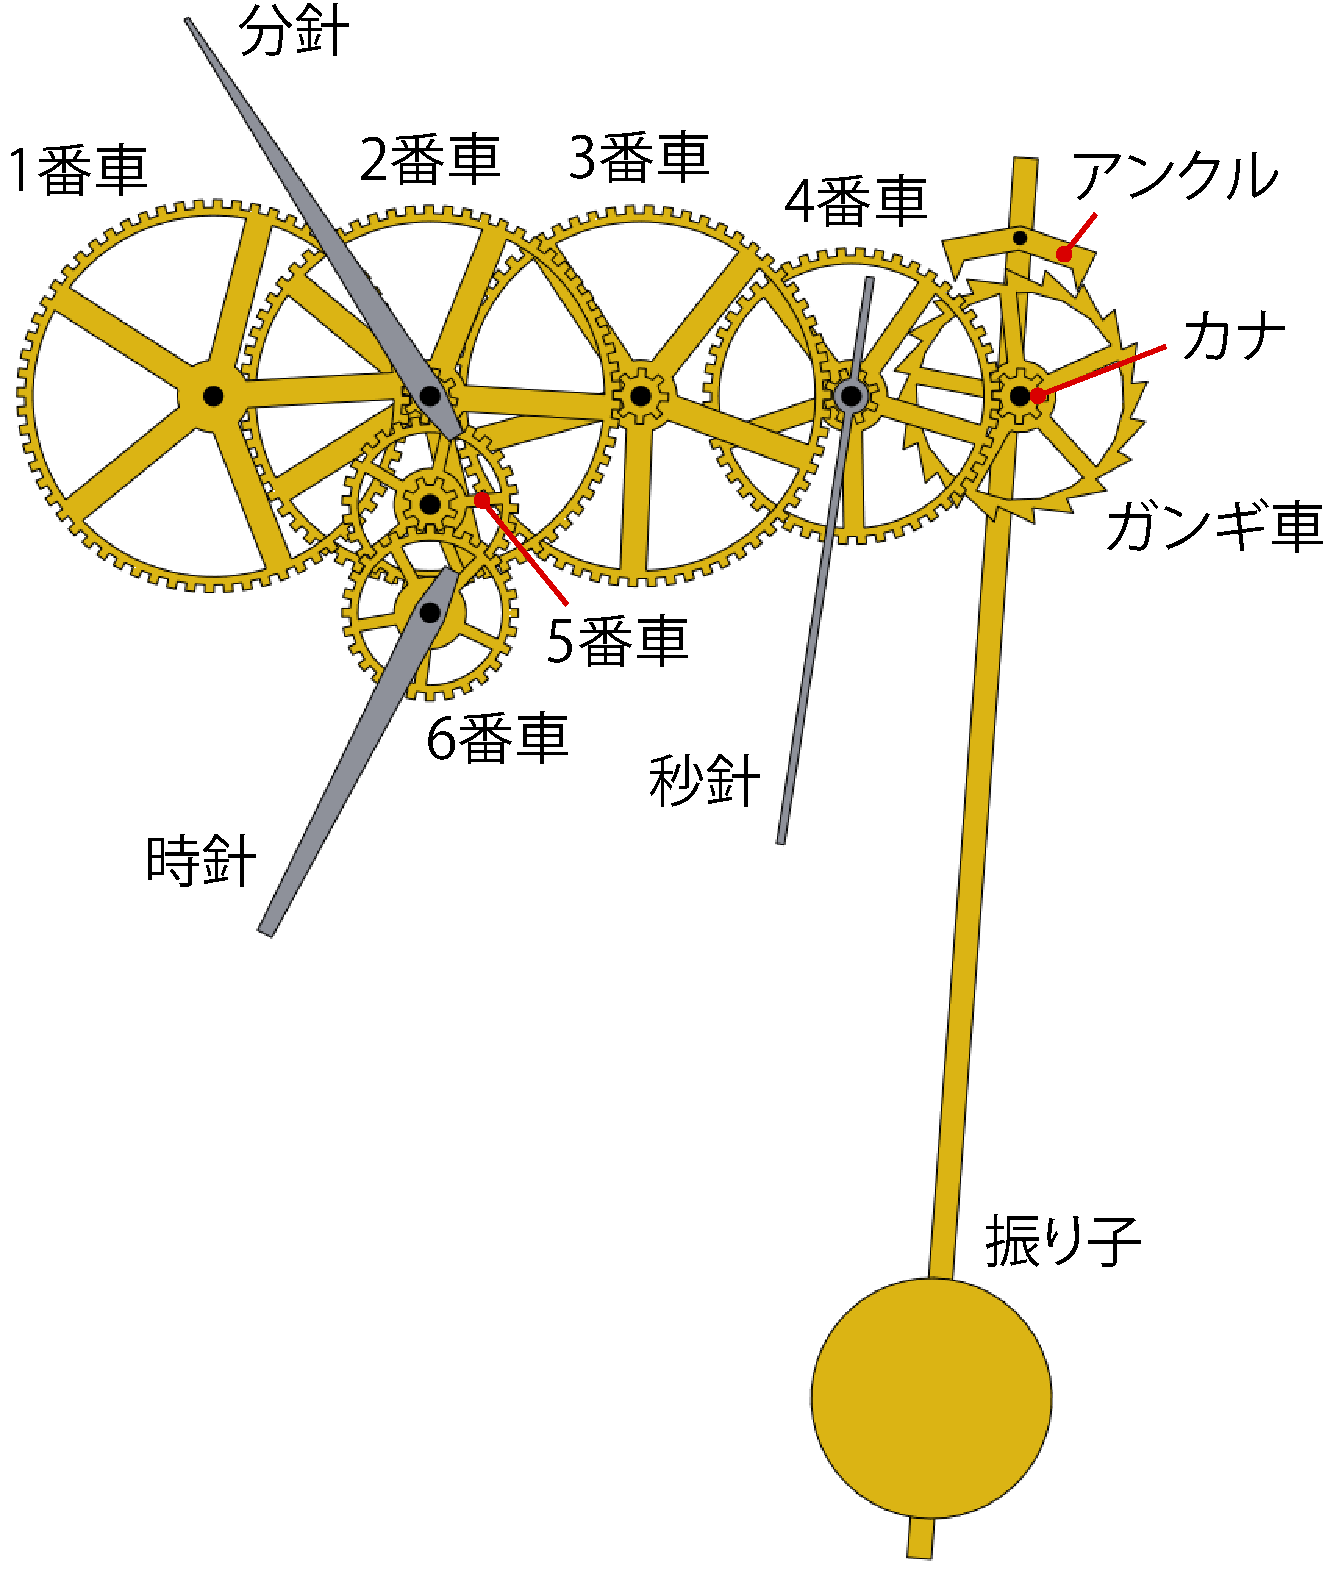
\includegraphics[width=12cm]{動作原理.pdf}
  \caption{振り子時計のパーツ}
  \label{fig:parts}
\end{figure}

図\ref{fig:parts}を見ると、1~6番車とガンギ車、アンクル、振り子で構成されていることが分かる。

2, 4, 6番車には、それぞれ分針、秒針、時針が取り付けられており、3, 5番車でそれぞれの回転速度の変換を行っている。
各歯車と、その中心にあるカナという歯車の歯数の比が、回転速度の比になる。
1番車は動力源となる歯車で、多くの場合は錘やモーター等によって動かされる。

しかしこれらのパーツだけでは、不安定な速度で周ってしまう。そこで、速度を一定に保つために振り子を利用する。
振り子には、振れ幅が十分小さければ、振れ幅に関係なく周期が一定になるという性質がある。
振り子の運動をガンギ車とアンクルで回転運動に変換することによって、精度良く回転速度を一定にすることができる。

なお、今回作成したプログラムでは、見栄えを良くするためにダミーの歯車を1つ追加した。これを0番車と呼ぶことにする。


\section{YAMLについて}
YAML (YAML Ain't a Markup Language)はXMLのように構造化されたデータを、XMLよりも人間に読み書きしやすい形にしたものである。
アプリケーションでbbs.dbを扱うために、ソースコード\ref{yml}ようにdatabase.ymlを作成する。
プログラム内でこのファイルを読み込むと、指定したデータベースを操作できるようになる。

\lstinputlisting[style=yaml,caption=database.yml,label=yml]{bbs/database.yml}


\section{ActiveRecordについて}
ActiveRecordはデータベースのレコードをオブジェクト指向言語のオブジェクトに対応させるライブラリである。
そうすることでオブジェクト指向言語でオブジェクトを操作すると、
内部的にデータベース管理システムのコマンドを発行し、
適切にデータベースを操作して結果を返してくれる。
SQLite3やMySQLなどのデータベース管理システムの違いをActiveRecordが吸収することで、
様々なデータベースをオブジェクト指向言語のオブジェクトへ対応させている。


\section{Webアプリケーションの構造}
今回作成したアプリケーションでは、処理部分と表示部分を分離させている。
処理本体はRubyで記述するが、表示はHTMLコードの中にRubyのコードを埋め込むことができるEmbedded Rubyで記述する。
Embedded Rubyは、表\ref{erb}に示すルールでRubyのコードを埋め込むことができる。

\begin{table}[H]
  \centering
  \caption{erbのルール}
  \label{erb}
  \begin{tabular}{|l|l|}
    \hline
    \chuo{記述} & \chuo{意味} \\ \hline \hline
    {\tt\verb|<%= code %>|}    & 囲まれた部分を実行して結果を埋め込む。         \\ \hline
    {\tt\verb|<% code %>|}     &  囲まれた部分を実行するが、結果は埋め込まない。 \\ \hline
    {\tt\verb|<%# comment %>|} &  囲まれた部分をコメントアウトする。            \\ \hline
  \end{tabular}
\end{table}

見た目を表すEmbedded Rubyのファイルは、viewsディレクトリの中に作成する。
アプリケーションフォルダのディレクトリ構造を図\ref{dir}に示す。

\begin{figure}[H]
\centering
\includegraphics[width=3.5cm]{file.pdf}
\caption{ディレクトリ構造}
\label{dir}
\end{figure}


\section{プログラムリスト}
図\ref{dir}で示した各プログラムのソースコードを、リスト\ref{main}-\ref{maincss}に示す。

\lstinputlisting[style=ruby,caption=bbs.rb,label=main]{bbs/bbs.rb}

\lstinputlisting[style=html,caption=main.erb,label=index]{bbs/views/main.erb}

\lstinputlisting[style=html,caption=error.erb,label=error]{bbs/views/error.erb}

\lstinputlisting[style=css,caption=style.css,label=style]{bbs/public/style.css}

\lstinputlisting[style=css,caption=main.css,label=maincss]{bbs/public/main.css}


\section{実装機能}
\subsection{投稿}
図\ref{f1}のように、名前とテキストを入力し、``Post''ボタンを押下すると掲示板にその内容が書き込まれる。
書き込まれた様子を図\ref{f2}に示す。
図\ref{f2}を見ると分かるように、投稿した日時も記録される。

\begin{figure}[H]
  \centering
  \includegraphics[width=6cm]{bbs02.png}
  \caption{投稿前の様子}
  \label{f1}
\end{figure}

\begin{figure}[H]
  \centering
  \includegraphics[width=6cm]{bbs03.png}
  \caption{投稿後の様子}
  \label{f2}
\end{figure}

入力フォームのHTMLは、main.erbの83行目以降に実装されている。
ボタンを押すと/newにPOSTし、それをサーバーサイドのプログラムbbs.rbの95行目でキャッチする。
ここでは、投稿識別ID、名前、テキスト、日時を取得し、ActiveRecordを介してデータベースに投稿を記録している。

\subsection{投稿の削除}
図\ref{f2}を見ると、投稿の横に``Delete''ボタンがあるのが分かる。
このボタンを押すと投稿が削除され、図\ref{f1}の状態に戻る。

``Delete''ボタンを押すと/delにリダイレクトされるように設定されており、このときbbs.rbの123行目以降が実行される。
当該のデータをデータベースから消去し、ページを再読み込みすることで投稿が削除される。

\subsection{サニタイズと改行}
\verb|<|や\verb|'|などの特殊な文字も入力できるように入力内容に対してサニタイズを行った。
サニタイズをすることで、HTMLタグを不正に実行される脆弱性を予防する効果もある。
また今回は、改行コードをHTMLタグ{\tt\verb|<br>|}に変換することで改行の入力を可能にした。

特殊な文字と改行を混じえた投稿の様子を図\ref{f3}に示す。
図\ref{f3}を見ると、各記号が正しく投稿されており、改行もされていることが分かる。

\begin{figure}[H]
  \centering
  \includegraphics[width=6cm]{bbs10.png}
  \caption{サニタイズと改行}
  \label{f3}
\end{figure}

\subsection{入力文字数制限}
main.erbの85, 88行目を見ると、input要素とtextarea要素にrequired, maxlength属性が付与されていることが分かる。
これにより、文字を入力していなくても文字数が多すぎても投稿出来ないようになっている。
図\ref{f4}は、文字を入力せずにPostボタンを押した時の挙動である。

\begin{figure}[H]
  \centering
  \includegraphics[width=6cm]{bbs06.png}
  \caption{入力必須フォーム}
  \label{f4}
\end{figure}

\subsection{ページ切り替え}
10件以上の投稿がある場合には、2ページ以降が追加される機能を実装した。
図\ref{f5}のように、すでに10件の投稿がある状態で投稿をすると2ページ目に投稿が追加される。
投稿された後の状態を図\ref{f6}に示す。
図\ref{f6}を見ると、新たに2ページ目が追加され、リダイレクトされていることが分かる。

\begin{figure}[H]
  \centering
  \includegraphics[width=6cm]{bbs07.png}
  \caption{10件の投稿がある状態}
  \label{f5}
\end{figure}

\begin{figure}[H]
  \centering
  \includegraphics[width=6cm]{bbs08.png}
  \caption{11件目の投稿}
  \label{f6}
\end{figure}

ページ番号はURLに指定できる。
指定されたページ番号ををbbs.rbの50行目で受け取り、そのページに相当する投稿を表示する。
なお、範囲外のURLが入力された場合は、エラーページを表示する。
エラーページが表示された様子を図\ref{f7}に示す。

\begin{figure}[H]
  \centering
  \includegraphics[width=6cm]{bbs11.png}
  \caption{エラーページ}
  \label{f7}
\end{figure}

\section{CSSの設定}
ページを見やすくするために、CSSを設定した。
全てのページで共通するスタイルをリスト\ref{style}のstyle.css, %
掲示板のページでのみ適用させたいスタイルを\ref{maincss}のmain.cssで設定することで、
メンテナンス性を向上させた。

CSSを設定していないページを図\ref{f8}に示す。
CSSを設定して色合いや間隔などを調整することで見やすくなることが分かる。

\begin{figure}[H]
  \centering
  \includegraphics[width=6cm]{bbs12.png}
  \caption{CSSを設定していないページ}
  \label{f8}
\end{figure}

\begin{thebibliography}{9}
  \bibitem{bib:1} 伊藤祥一, ``Springs of C 楽しく身につくプログラミング'', 森北出版株式会社, 2017, pp. 109--110.
  \bibitem{bib:2} ``Pendulum clock'', Wikipedia, \texttt{https://en.wikipedia.org/wiki/Pendulum_clock}, 参照2019/12/5.
\end{thebibliography}

\end{document}
